\chapter{Banco de dados}
\label{banco}

\todo{atualizar features}
\todo{colocar os algoritmos de criação de feature - TCC do scholles}

Como mencionado na subseção \ref{dataset}, a criação de um banco de dados ou \textit{dataset} é fundamental para o treinamento de um algoritmo de aprendizado de máquina. No conjunto de dados devemos especificar quais são os dados de entrada que o algoritmo irá receber e qual a saída esperada para aquela entrada, a partir disso o programa deve fazer uso da função de custo para ajustar os parâmetros do modelo de forma a conseguir acertar a saída com a maior precisão.

Neste trabalho, o banco de dados está no formato tabular, isto é, as informações estão dispostas em uma tabela. Cada linha da tabela possui um conjunto de \textit{features} (os dados de entrada) e um \textit{label} (o rótulo ou saída desejada). Este tipo de conjunto de dados é chamado de \textit{dataframe}, uma estrutura de dados bidimensional com os dados alinhados de forma tabular em linhas e colunas.

Como foi dito na seção \ref{cap_intr}, o conjunto de dados é retirado de uma fonte pública disponível na internet, o Amazon Dashboard do GFED. Pelo site é possível fazer o download de um arquivo \textit{.zip} com diferentes tipos de arquivos que contém um mapa da região da floresta amazônica na América do Sul e os diversos eventos de fogo que aconteceram na região desde 2020.

\subsection{\textit{Shapefile}}
\label{sec:shp}

O arquivo obtido é do tipo \textit{shapefile}, um formato de armazenamento de dados de vetor para armazenar a posição, forma e atributos de feições geográficas. Este tipo de arquivo pode ser aberto por meio de \textit{softwares} gratuitos como o QGIS, utilizado para visualização de dados GIS (Sistema de Informação Geográfica), para captura de dados, para análise avançada de GIS e para apresentações na forma de mapas, atlas e relatórios sofisticados \cite{qgis}. Um GIS integra informações descritivas a um mapa, eles incluem imagens, feições e mapas base vinculados a planilhas e tabelas.

Ao abrimos o \textit{shapefile} no QGIS, primeiro nos deparamos com uma imagem das queimadas que foram analisadas pelo GFED na região que contém a floresta amazônica desde 2020 até 31 de maio de 2022, como mostrado na figura \ref{fig:mapashp}. Com o projeto aberto, podemos escolher visualizar a tabela de atributos que acompanha o mapa, que está representada na figura \ref{fig:tabat}. A tabela de atributos contém as feições relativas a cada polígono que compõe a imagem do mapa da América do Sul. Os atributos que fazem parte da tabela são:

\begin{figure}[htb]
	\centering
	\begin{minipage}{0.9\linewidth}
		\centering
		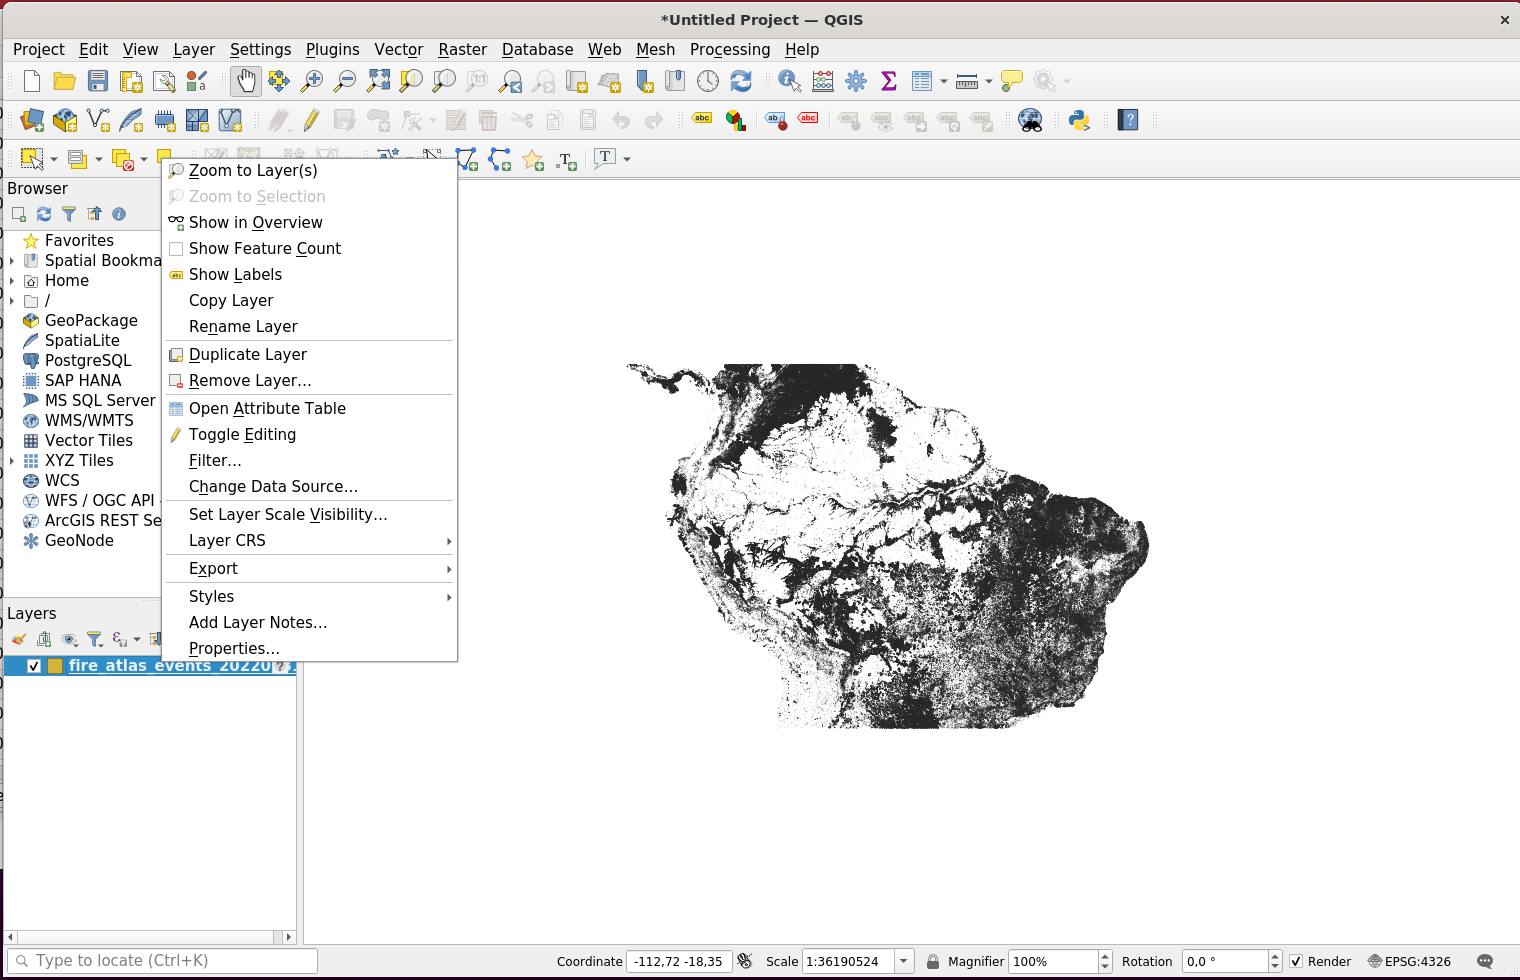
\includegraphics[width=\linewidth]{tg1/figuras/mapa.png}
		\caption{Mapa da América do Sul com os eventos de fogo detectados} \label{fig:mapashp}
	\end{minipage}
\end{figure}

\begin{figure}[htb]
	\centering
	\begin{minipage}{0.9\linewidth}
		\centering
		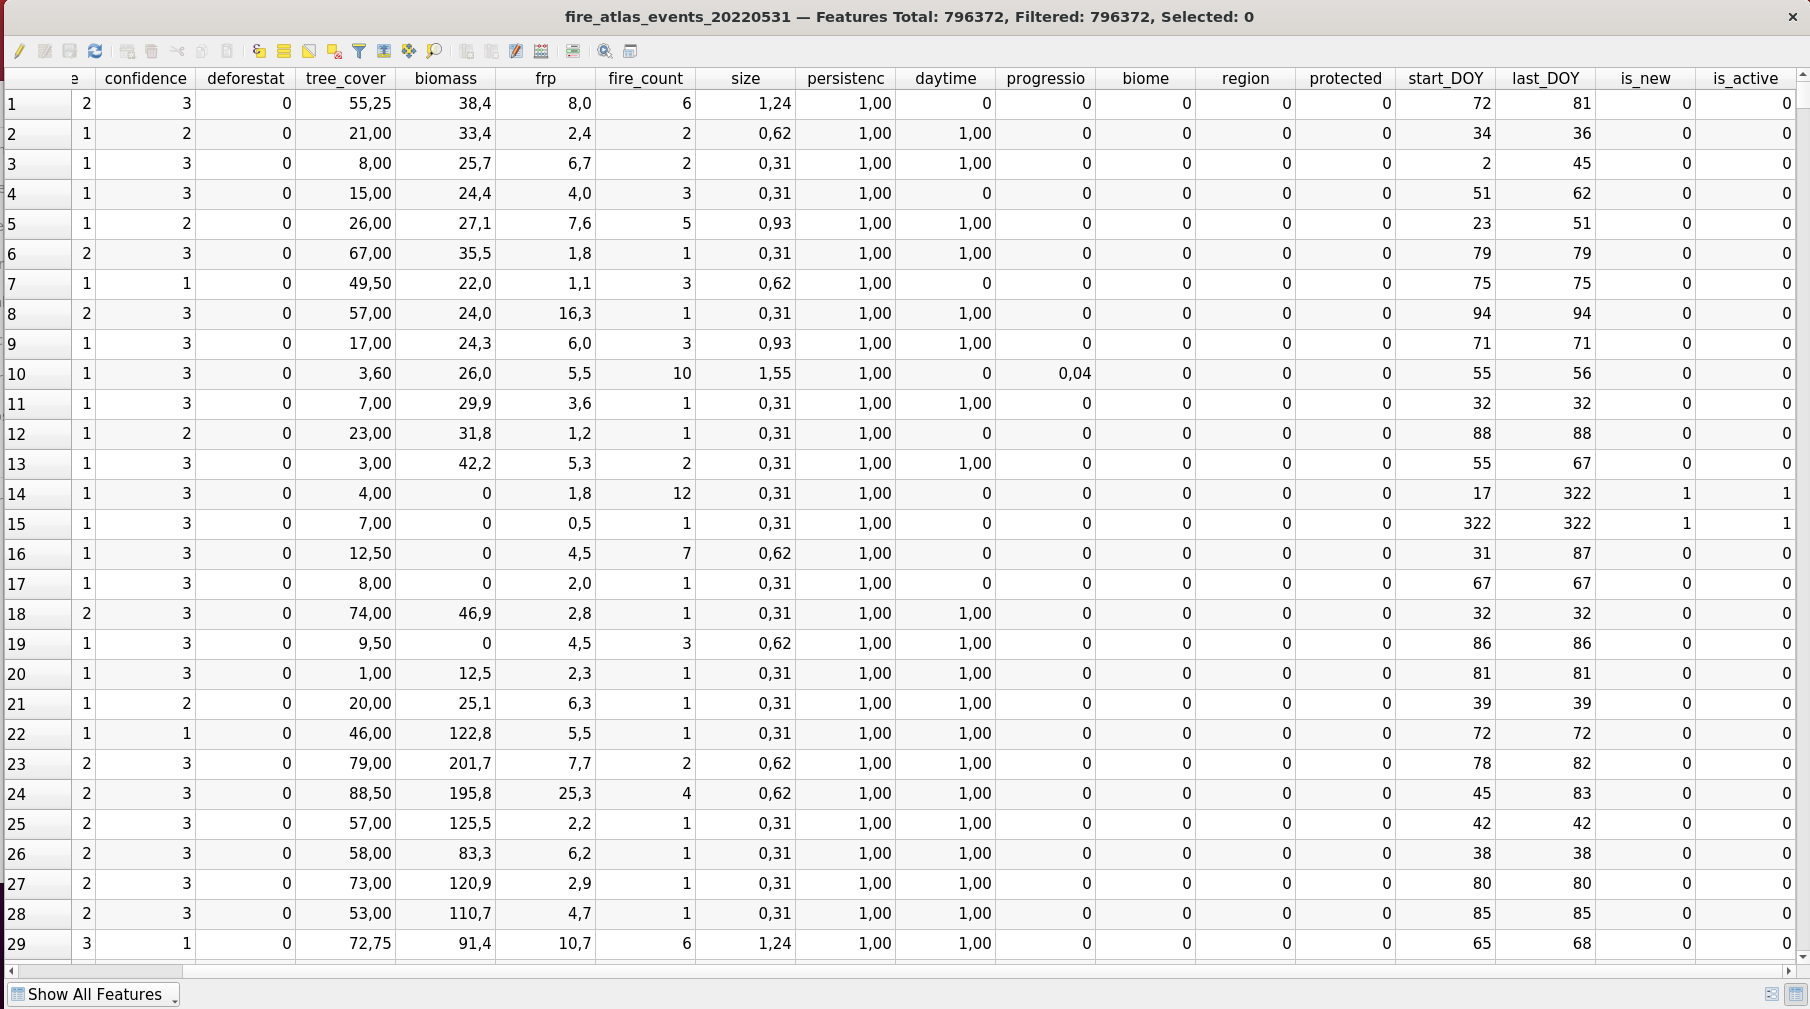
\includegraphics[width=\linewidth]{tg1/figuras/tabela_atributos.png}
		\caption{Tabela de atributos do \textit{shapefile}} \label{fig:tabat}
	\end{minipage}
\end{figure}

\begin{enumerate}
\item \textbf{id\_event\_1}: Representa o código de identificação interno de um evento de fogo catalogado pelo sistema. Detecções distintas mas consideradas como um mesmo evento recebem a mesma identificação.
\item \textbf{delta\_area}: Variação da área coberta pelo incêndio em kilometros quadrados.
\item \textbf{q\_focos}: Quantidade de focos de incêndio detectados pelo sistema como pertencendo ao mesmo evento de fogo.
\item \textbf{qtd\_passag}: Quantas passagens de satélites ocorreram por este evento. Como se trata de 4 pares de satélite em órbitas polares, pode-se ter até 8 detecções por dia \cite{painel-fogo}.
\item \textbf{frp\_med}: \textit{Fire Radiative Power} ou FRP é um dado relativo ao sensor MODIS (\textit{Moderate Resolution Imaging Spectroradiometer}. Trata-se de uma técnica para quantizar biomassa queimada medindo a radiação de energia infravermelha \cite{NASA\_MODIS}.
\item \textbf{area\_passa}:
\item \textbf{delta\_t\_ho}: Tempo acumulado em horas entre detecções.
\item \textbf{p\_norm}:
\item \textbf{ve\_expansa}: Velocidade estimada de expansão do incêndio.
\item \textbf{areakm2\_UC}:
\item \textbf{perc\_in\_UC}:
\item \textbf{areakm2\_IN}:
\item \textbf{perc\_in\_IN}:
\item \textbf{deter\_area}:
\item \textbf{deter\_days}:
\item \textbf{deter\_perc}:
\item \textbf{tree\_cover}: Cobertura de árvore, métrica referente à porcentagem da área que é coberta por copas de árvores ou vegetação alta.
\item \textbf{a\_cover\_X and p\_cover\_X}: (where X can be 3, 4, 5, 9, 11, 12, 15, 20, 21, 23, 24, 25, 29, 30, 32, 33, 39, 40, 41, 48, 62)
\item \textbf{biomass\_AG}:
\item \textbf{biomass\_GS}:
\item \textbf{a\_terr\_pri and p\_terr\_pri}:
\item \textbf{a\_terr\_pub and p\_terr\_pub}:
\item \textbf{a\_terr\_unk and p\_terr\_unk}:
\item \textbf{area\_CAR}:
\item \textbf{per\_CAR}:
\end{enumerate}


Dos dados listados acima, apenas 18 são disponibilizados diretamente pelos servidores do CENSIPAM. Os demais dados têm de ser produzidos a partir de outros conjuntos de dados disponibilizados por diferentes entidades. 

A produção destes dados envolvem o cruzamento com dados de diversas outras entidades. Sua produção se dá pelo cálculo da intersecção geográfica dos eventos de fogo e diversos mapas disponibilizadas pelas entidades Terrabrasilis \cite{terrabrasilis}, MapBiomas \cite{MapBiomasQueimadas} e GFED \cite{gfed}. 

A partir das coordenadas dos focos de incêndio, é possível de se fazer uma comparação com diversos mapas para se encontrar intersecções com áreas de interesse. Por exemplo, dados relativos à proximidade à áreas de conservação ambiental e áreas indígenas são produzidos pelo cruzamento com os dados disponíveis pelo Terrabrasilis. A plataforma disponibiliza arquivos no formato "shapefile" contendo as geometrias das delimitações geográficas de cada área, que são então comparadas as coordenadas dos eventos detectados para se calcular se há intersecção e qual a porcentagem desta intersecção, isto é, o quanto da área do incêndio está contida dentro dessas delimitações.

Status de desmatamendo - DETER

Áreas Públicas, Privadas, Desconhecidas e Áreas de Cadastro Ambiental Rural

\todo[]{achar um jeito de escrever bem essa parte sem entrar muito em detalhes pq é tcc do xoles}


\subsection{\textit{Dataframe}}

Para converter o conteúdo da tabela de atributos em um \textit{dataframe}, faz-se necessário o uso das bibliotecas \textit{geopandas} e \textit{pandas} do \textit{python}. \textit{Pandas} é uma ferramenta de análise e manipulação de dados, e \textit{geopandas} estende os tipos de dados usados pelos \textit{pandas} para permitir operações espaciais em tipos geométricos. O que fazemos então é primeiro abrir o arquivo do tipo \textit{shapefile} usando \textit{geopandas} para criar um \textit{GeoDataFrame} e então usar uma função da biblioteca \textit{pandas} para convertê-lo em um \textit{dataframe} normal com as \textit{features} que iremos utilizar como entrada para os algoritmos de aprendizado de máquina.

\section{Análise das \textit{features}}

\todo{isso ainda é válido? utilizamos todas estas features?}

Ao todo são utilizadas 17 \textit{features} diferentes para realizarmos a classificação do tipo de fogo, que estão descritas na subseção \ref{sec:shp} (cluster\_ID não é utilizado). Nem sempre todas as informações que entregamos para um algoritmo de aprendizado de máquina são úteis para a previsão, o que explica não utilizarmos o cluster\_ID, pois se cada evento de fogo possui um número de identificação diferente, esse número nada diz a respeito sobre qual o tipo de queimada que ocorreu. Podemos fazer uma correlação entre cada tipo de dado fornecido e os tipos de fogo, observando assim quais informações são mais descritivas para o algoritmo, quais delas são mais úteis para separar os 4 tipos.

Para podermos observar a relação que cada \textit{feature} possui com a saída, foram feitos diversos gráficos de dispersão em 3 dimensões que combinam o efeito que até 3 \textit{features} em conjunto podem ter para separar cada tipo de queimada em nuvens. Os gráficos estão dispostos nas figuras .

\begin{multicols}{2}

\begin{figure}[H]
    \caption{Biome x Region x Protected}
     
    \centering 
    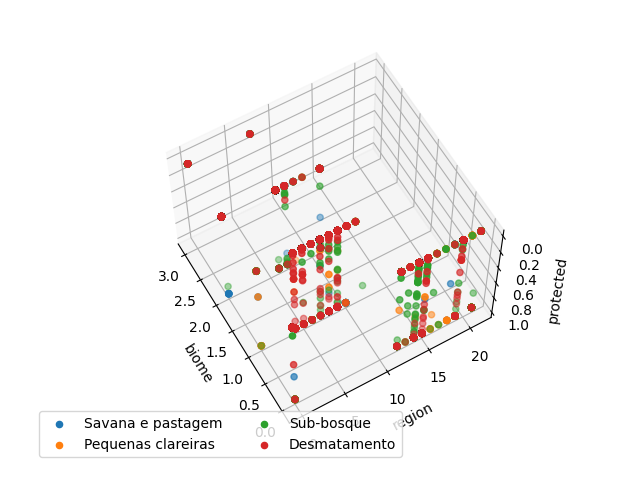
\includegraphics[width=1.1\linewidth]{tg1/figuras/biomexregionxprotected--120-30.png}
    \label{figura:one}
\end{figure}
        
\begin{figure}[H]
    \caption{Biome x Region x Protected}
     
    \centering 
    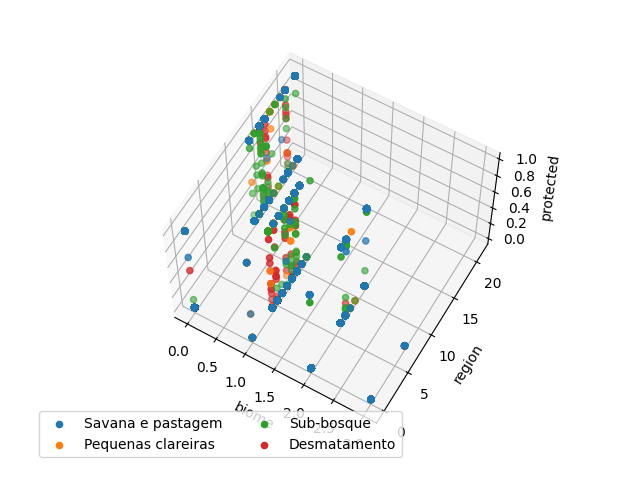
\includegraphics[width=1.1\linewidth]{tg1/figuras/biomexregionxprotected-60--60.png}
    \label{figura:two}
\end{figure}

\begin{figure}[H]
    \caption{Deforestat x Tree cover x Biomass}
     
    \centering 
    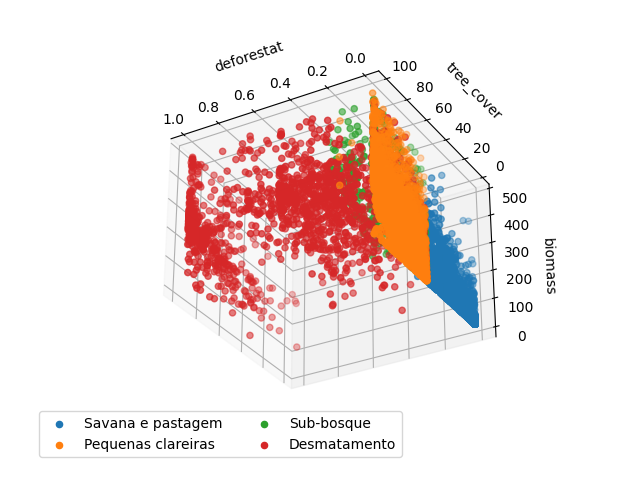
\includegraphics[width=1.1\linewidth]{tg1/figuras/deforestatxtree_coverxbiomass---30--120.png}
    \label{figura:three}
\end{figure}

\begin{figure}[H]
    \caption{FRP x Detections x Size}
     
    \centering 
    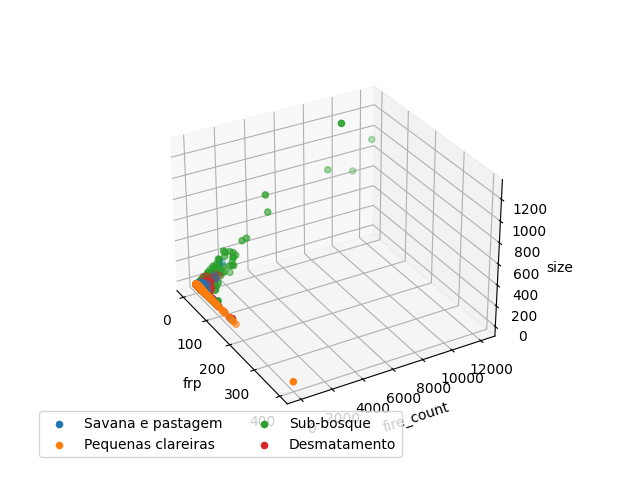
\includegraphics[width=1.1\linewidth]{tg1/figuras/frpxfire_countxsize-30--30.png}
    \label{figura:four}
\end{figure}

\begin{figure}[H]
    \caption{Persistence x Daytime x Progression}
     
    \centering 
    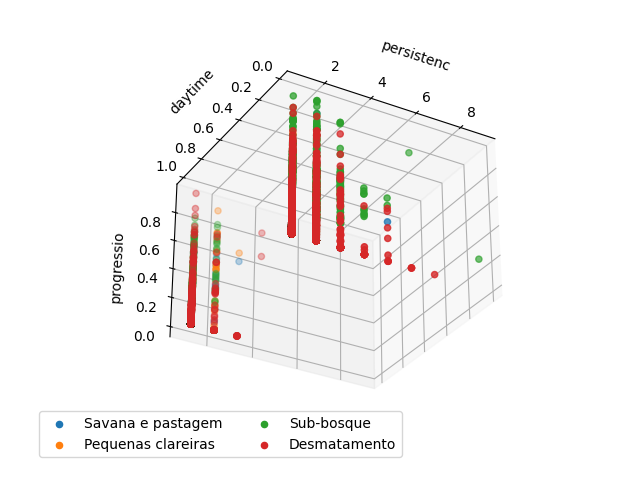
\includegraphics[width=1.1\linewidth]{tg1/figuras/persistencxdaytimexprogressio--30--120.png}
    \label{figura:five}
\end{figure}

\begin{figure}[H]
    \caption{Start day x Is new x Is active}
     
    \centering 
    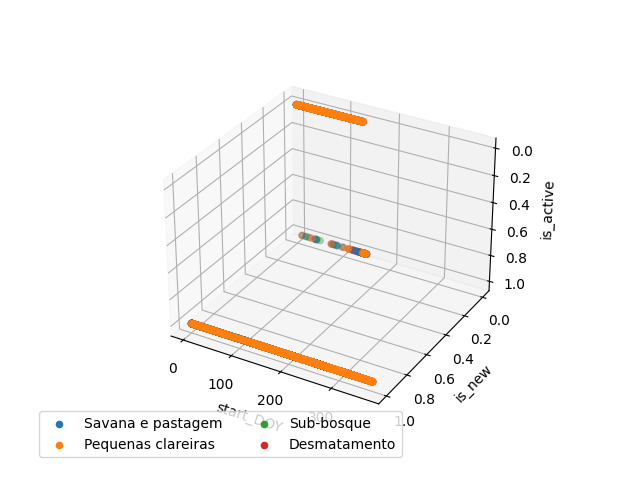
\includegraphics[width=01.1\linewidth]{tg1/figuras/start_DOYxis_newxis_active--150--120.png}
    \label{figura:six}
\end{figure}

\begin{figure}[H]
    \caption{Start day x Is new x Is active}
     
    \centering 
    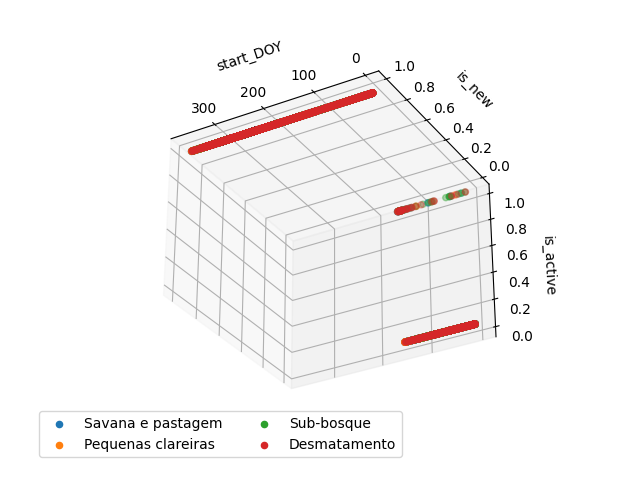
\includegraphics[width=1.1\linewidth]{tg1/figuras/start_DOYxis_newxis_active--30-120.png}
    \label{figura:seven}
\end{figure}
            
\end{multicols}

Podemos observar através dos gráficos porque os tipos de fogo de savana (0) e pequenas clareiras (1) possuem precisão tão alta, dados como \textit{tree cover}, \textit{deforestat}, \textit{frp}, \textit{fire count} e \textit{biomass} em conjunto são capazes de delimitar fortemente esses dois tipos. O desmatamento (4) e sub-bosque (3) apresentam maior diluição um com o outro e com os outros tipos, o que explica a maior dificuldade dos algoritmos em prevê-los corretamente, além do que podemos ver na tabela \ref{tab:rf} que eles são os dois tipos menos presentes no \textit{dataset}, e os algoritmos costumam ter maior facilidade para prever corretamente as saídas mais comuns.



